\section{Le matériel}

\subsection{Intérêt}
\begin{frame}{Pourquoi existe-t-il des clavier de 5~à~500€~?}
    \begin{itemize}
        \item Les claviers standards héritent des lourdeurs du passé: touches
        en diagonale, position  du retour à la ligne, du backspace, … \pause
        \item Il existe des claviers ergonomiques, bien plus pratiques (touches
        mécaniques, clavier matriciel, dont la forme s’adapte aux mains…).
    \end{itemize}
\end{frame}

\subsection{Forme générale}
\begin{frame}{Forme générale}{Classique}
	\begin{center}
		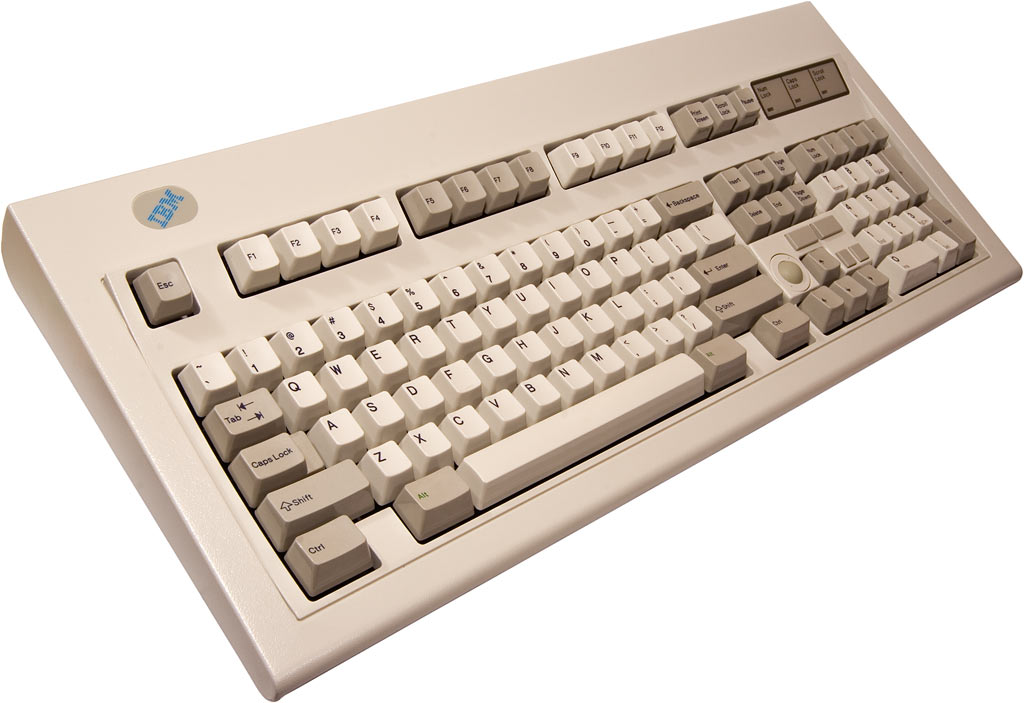
\includegraphics[scale=0.28]{images/hard_modelm}
	\end{center}
\end{frame}

\begin{frame}{Forme générale}{Matriciel}
	\begin{center}
		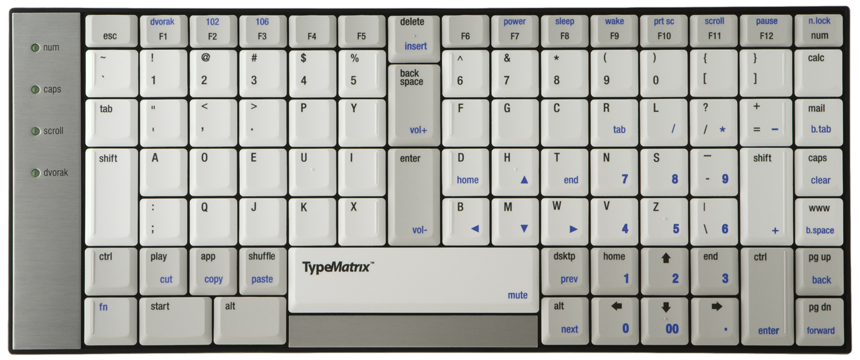
\includegraphics[scale=0.25]{images/2030-dvorak} \\~\\
		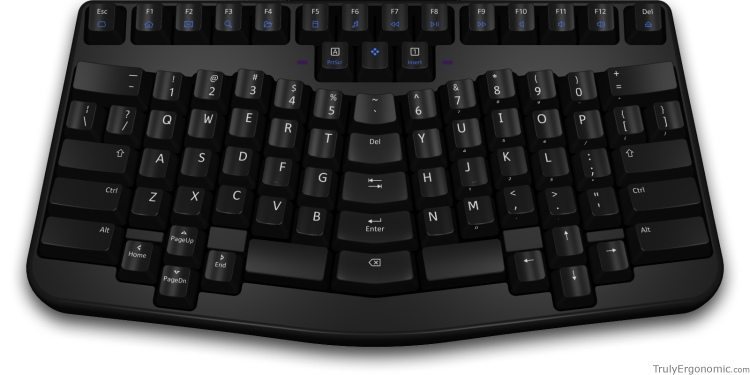
\includegraphics[scale=0.25]{images/t_e_keyboard}
	\end{center}
\end{frame}

\begin{frame}{Forme générale}{Ergonomique}
	\begin{center}
		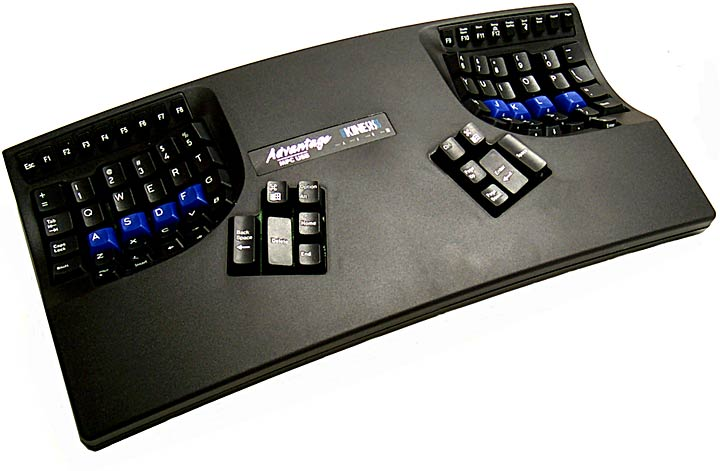
\includegraphics[scale=0.25]{images/hard_kinesis} ~
		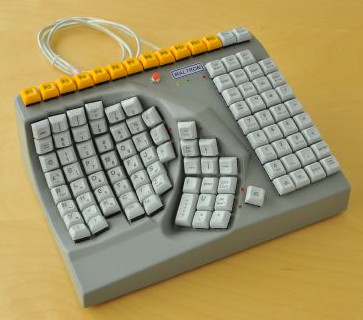
\includegraphics[scale=0.4]{images/hard_maltron}
	\end{center}
\end{frame}

\subsection{Mécanismes de touches}
\begin{frame}{Linéaire ou tactile}
	\begin{center}
		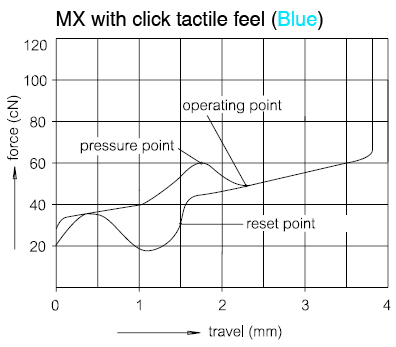
\includegraphics[scale=0.4]{images/hard_bluecurve} ~
		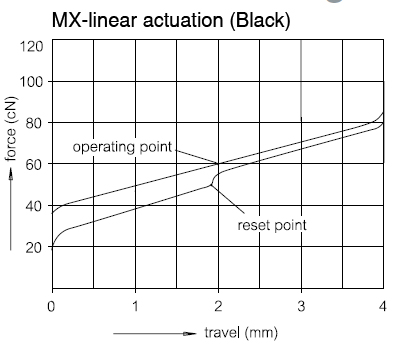
\includegraphics[scale=0.4]{images/hard_blackcurve}
	\end{center}
	\begin{itemize}
		\item Courbe de force en fonction du poids appliqué.
	\end{itemize}
\end{frame}

\subsection{Mécanisme des touches}
\begin{frame}{Rubber Dome}
	\begin{center}
		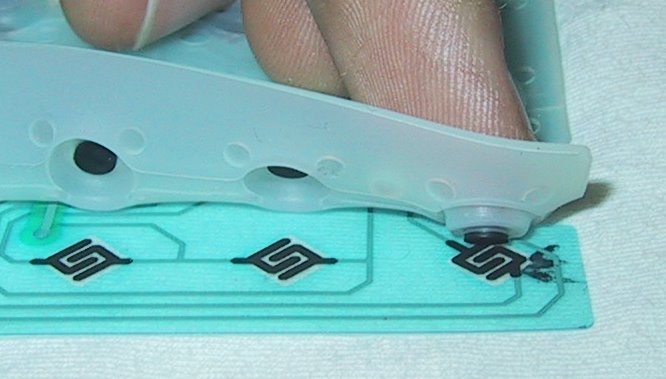
\includegraphics[scale=0.4]{images/hard_rubberdome}
	\end{center}
	\begin{itemize}
		\item Linéaire, très répandu, utilisé par 90\% des claviers,
		\item tous les claviers à moins de 40€, Keytronics\dots
	\end{itemize}
\end{frame}

\begin{frame}{Scissor Switch}
	\begin{center}
		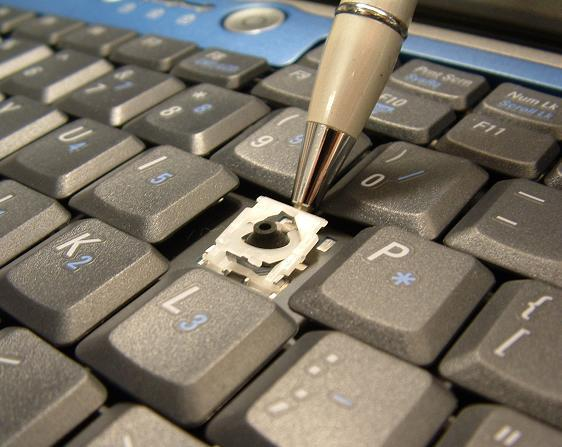
\includegraphics[scale=0.3]{images/hard_scissor}
	\end{center}
	\begin{itemize}
		\item Linéaire, silencieux, très répandu, fait mal aux doigts.
		\item La plupart des claviers plats (laptop, Apple\dots).
	\end{itemize}
\end{frame}

\begin{frame}{Buckling Spring}
	\begin{center}
		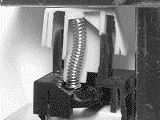
\includegraphics[scale=0.8]{images/hard_buckling} ~
		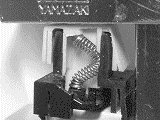
\includegraphics[scale=0.8]{images/hard_buckling2}
	\end{center}
	\begin{itemize}
		\item Tactile, bruyant,
		\item IBM model~M, Unicomp.
	\end{itemize}
\end{frame}

\begin{frame}{Cherry MX}
	\begin{center}
		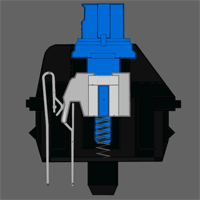
\includegraphics[scale=0.5]{images/hard_cherryblue} ~
		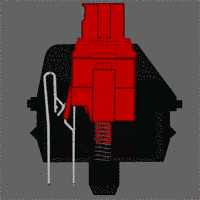
\includegraphics[scale=0.5]{images/hard_cherryred}
	\end{center}
	\begin{itemize}
		\item Red~: linéaire, silencieux,
		\item Black~: linéaire, silencieux,
		\item Blue~: tacticle, bruyant,
		\item Brown~: tacticle, silencieux.
		\item Utilisées par les Truly Ergonomics, Das Keyboard, Filco, Kinesis,
		certains SteelSeries et Razer\dots
	\end{itemize}
\end{frame}

\begin{frame}{Autre…}
	\begin{center}
		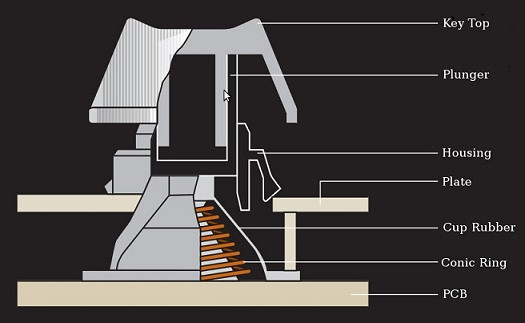
\includegraphics[scale=0.4]{images/hard_topre}
	\end{center}
	\begin{itemize}
		\item Topre~: tactile, silencieux. Happy Hacking Keyboard\dots
		\item Alps~: tactile, silencieux. Certains Kinesis, certains Dell\dots
	\end{itemize}
\end{frame}
